% Especificaciones del tamaño de letra, tamaño de hoja, márgenes, librerias, etc.
\documentclass[12pt, letterpaper]{article}
\usepackage[english]{babel}
\usepackage{fancyhdr}
\usepackage[utf8]{inputenc}
\usepackage[T1]{fontenc}
\usepackage{amsmath}
\usepackage{graphicx}
\usepackage{subcaption}
\usepackage[hidelinks]{hyperref}
\usepackage{url}
\usepackage{amssymb}
\usepackage{float}
\usepackage[margin=1in]{geometry}
\renewcommand{\baselinestretch}{1.5}

% Enlace Bibliografía
\usepackage{csquotes}
\usepackage[notes,backend=biber]{biblatex-chicago}
\addbibresource{referencias.bib}

% Titulo, autores, fecha.
\title{Technical Report \#1}
\author{Carlos A. Vásquez Castañeda \and 1155057 \and Group 392}
\date{November 6, 2019}
\pagestyle{fancy}
\fancyhf{}
\rhead{Aircraft Elements Design}
\lhead{Technical Report \#1}
\rfoot{\thepage}


% Inicio del documento
\begin{document}
\maketitle
\section*{Introduction}

The overall assembly of any product needs to be done in an ordered and logical manner, and it is of utter importance to consider the manufacturing methods and other physical constrains that might be encountered as the model is launched into production. For these reasons, this technical report aims to explain the process of assembling a standard jet engine, with most parts of it and the logic behind the placement and of the pieces, aswell as the mechanics of the individual parts and the engine as a whole.

\section*{Assembly}
\subsubsection*{General Layout of the Engine}
The assembly process starts with a fixed piece. This reference will be where all the other parts of the assembly will be connected and where all the constrains will be made (with respect to this fixed part). Considering these characteristics, the best fixed piece we can choose for this design is the shaft. The shaft will be the part that will connect every other piece together and, considering that in the actual physical model the shaft delivers the power to other components, it is logical to think of it as the fixed part of the assembly.

To make sense of the assembly before adding parts, we need to understand a little about jet engines. Generally jet engines can be divided into six parts. The air intake, the compressor stage, the diffuser stage, the combustion stage, the turbine stage and the exhaust stage.

The whole point of a jet engine is to generate thrust and help lift the aircraft. Giving these stages, we can order them as shown in figure 1.

\begin{figure}[H]
	\centering
	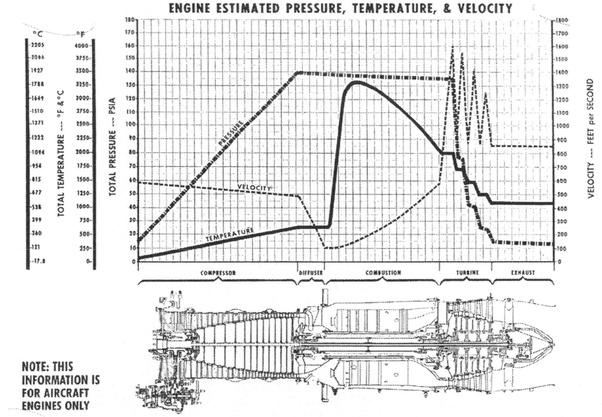
\includegraphics[width=0.9\textwidth]{plot.jpeg}
	\caption{Pressure, velocity and temperature of the air going through the jet engine at different stages.}
\end{figure}

\subsubsection*{Shaft and Fan Blade}
For the air intake (which comes right before the compressor stage), we need a way of generating a pressure difference so air can flow into the jet engine. The piece which is in charge of this is the high bypass fan blade. This part of the engine is right at the beggining of it and is attached to the shaft directly. The way we constrain the fan blade is by a concentricity constrain with the shaft and a contact constraing with one of the faces of the fan blade and une face of the shaft. This way, only one degree of freedom is left for the fan blade, which is the rotation with respect to the y-axis, which is the same as the rotation with respect to the shaft axis. Shown in figure 2 is the assembly at this point in time.

\begin{figure}[H]
	\centering
	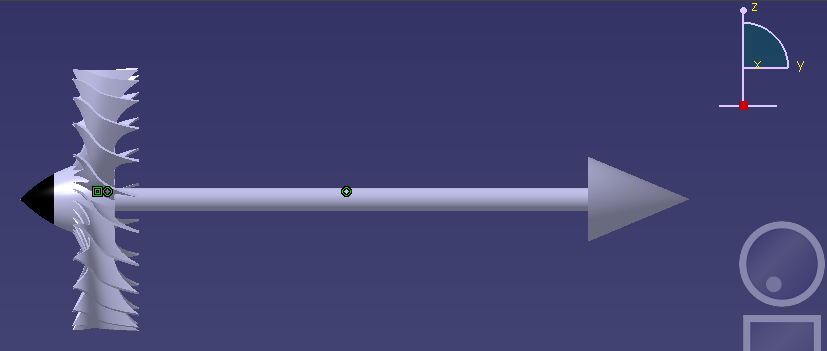
\includegraphics[width=0.9\textwidth]{1.png}
	\caption{Shaft and fan blade constrained with each other.}
\end{figure}

The orientation of the fan blade is quite easy to determine, as the black tip of it is facing outwards, which indicates it will pull air in the opposite direction. Also the way the blades are oriented determine the flow of air into the engine itself.

\subsubsection*{Compressor}
Afterwards comes the compression stage. Many engines differ as to what kind of compression they use and how many substages this stage has. It depends on the design and the function/type of engine. Compressors generally are either axial or centrifugal. The axial ones compress air in the same axis as the axis of the shaft and the centrifugal ones compress air by spining the air and getting it into the sides of the chamber, which accelerates it. The compotent of the compressor which takes care of the rotation/acceleration of air is called the \textit{rotor} in axial compressors and the \textit{impeller} in centrifugal compressors.

Accelerating air is just one part of the process of compression, the other is to suddenly stop it to pack it together and elevate the pressure. As it is seen in figure 1, there is a decrease in velocity when the compressor stage is at play. This is counterintuitive as we have said that the air is being accelerated. However, after the acceleration, the air comes to a sudden stop and it is compressed. The compotent which brakes the air is called the \textit{stator} in axial compressors and the \textit{diffuser} in centrifugal compressors. 

Shown in figure 3 is the way the compressor is layed out in the shaft. As we can see, we have two components, and this is because we have two phases in the compression stage. The first phase (the left one) is the low pressure compressor. At this point air is compressed but not totally. We have two compression phases because this way is more efficient, we save power and we limit the pressure diferential. The last phase at the right is the high pressure compressor, which takes the air and finishes its compression for the next stage of the engine.


\begin{figure}[H]
	\centering
	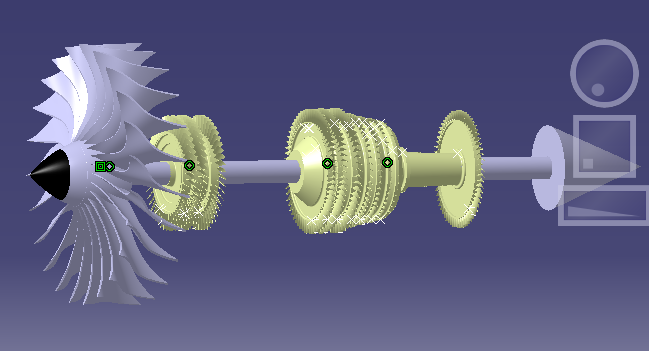
\includegraphics[width=0.9\textwidth]{2.png}
	\caption{Low pressure and high pressure compressor attached to the shaft.}
\end{figure}

As with the fan blade, the compressors need to be concentric to the shaft's longitudinal axis, therefore making a concentricity constrain we are left with only two degrees of freedom, which are the rotation with respect to the y-axis and the movement in the same axis. When the assembly is finished, the movement of these components in the y-axis is undesired. Later on the measurements of the distances between components will be defined, but for now is redundant as the other parts of the engine haven't been added.

\subsubsection*{Planetary Gear and Bearing}
The bearing and planetary assembly are represented by the pieces shown in figure 4. the leftmost piece is the planetary assembly, which features three gears, and the bearing is the piece to the right of the planetary assembly in figure 4. This bearing isn't the actual model of the physical bearing, but rather a representation of it. We don't need to add the whole model as it will only costs us CPU when manipulating the model. The planetary assembly helps to mantain a certain velocity and to give power to other parts of the design. The bearing reduces the friction when the shaft is spinning, which lets us have a greater efficiency.

The way these pieces where constrained is the same as the compressors. As for the planetary assembly in particular, a coincidence constrain was made with one of the faces of the sun gear. This was to assure the right orientation of the planetary assembly. Therefore, the way of making this constrain is by making a face of the sun gear coincide with the one of the shaft (the cylindrical one).

\begin{figure}[H]
	\centering
	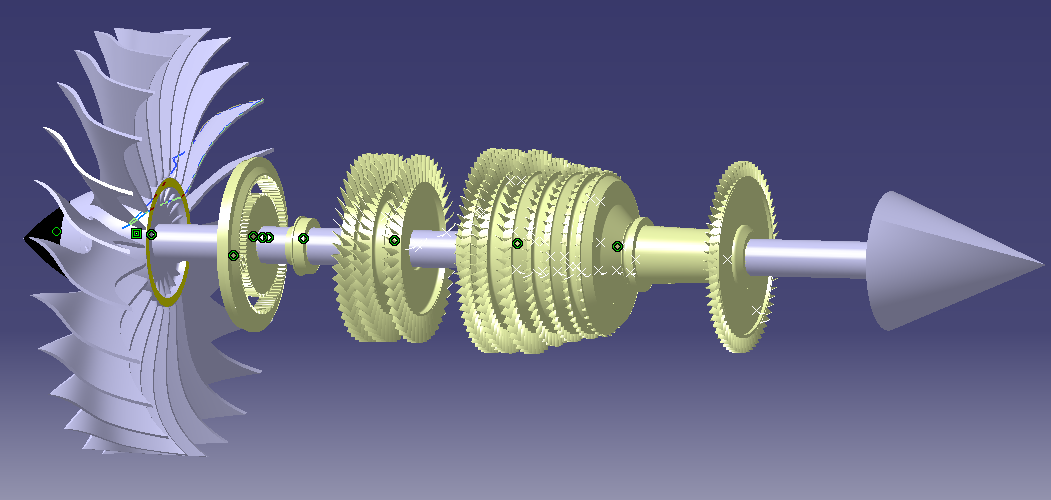
\includegraphics[width=0.9\textwidth]{3.png}
	\caption{Planetary assembly and bearing, constrained to the same longitudinal axis as the shaft.}
\end{figure}

\subsubsection*{Combustor}

After adding the planetary assembly, bearing and compressors, we continued with the combustor. This piece is essential to the engine as it determines its efficency. The last stage of the engine is the turbine stage, and the turbine needs to draw power form somewhere in order to turn, and so, the combustor is in charge of combining fuel with highly pressurised air and ignite it so it can produce high temperature gas that will go through the turbine, giving it power and it will also provide thrust when passed through a nozzle.

Before we've made the remark that the combustor decides the efficency of the engine as a whole. The way this works is by designing the combustion chamber. It plays a crucial role in determining most of the engine's operating characteristics, such as fuel efficency, levels of emissions and the transient response (the response to changing conditions such as fuel flow and air speed).

\begin{figure}[H]
	\centering
	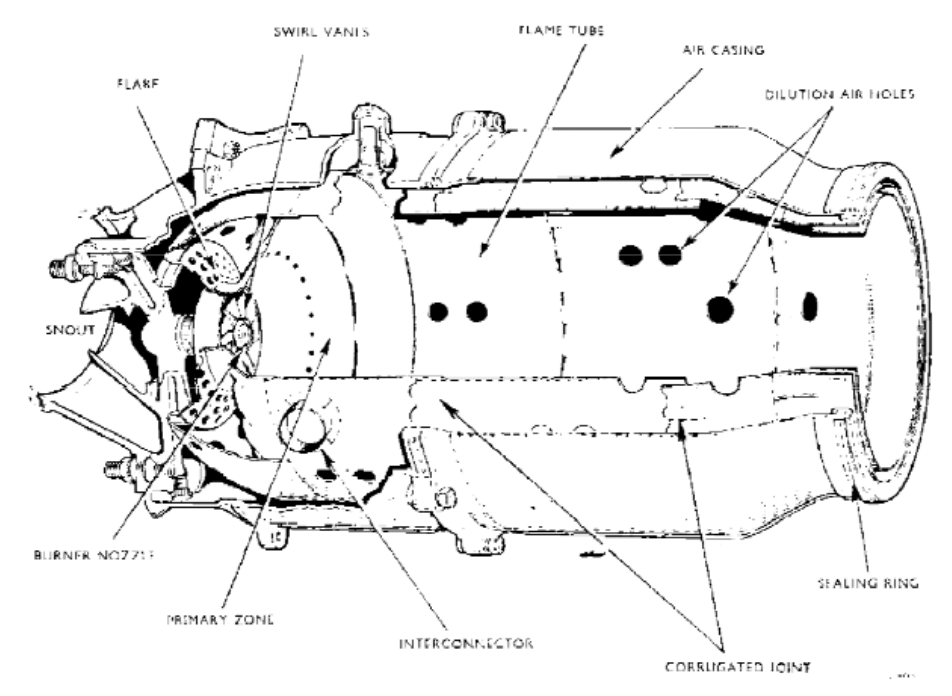
\includegraphics[width=0.9\textwidth]{comb.png}
	\caption{Parts of the combustion chamber.}
\end{figure}

The general layout of the combustion chamber is shown in figure 5. The air flows into the nozzle and the goes into the flare, where it is slowed down and compressed a little more (if we take a look at figure one, as the aire comes into the combustion chamber, when it gets to the flare it has the highest pressure in all of the engine). Then in the primary zone, the air gets mixed with the fuel and gets ignited. Later, as there is a percentage of air which goes into the secondary flow, that air goes into the inside of the chamber via the dilution holes, which give the flame stability and enriches the already ignited air in the primary zone. Also, this secondary flow makes an air casing which protects the metal encasing the whole combustion chamber and taking care of the high temperatures made by the ignition, making an air pocket insulation.

There are three types of combustion chambers, but they all operate in the same way. There is the can type, the cannular type and the annular type. For all extensive purposes, the combustor type used in this engine is an annular type, as it has more efficiency than the other ones, althought it is more difficult to mantain.

\begin{figure}[H]
	\centering
	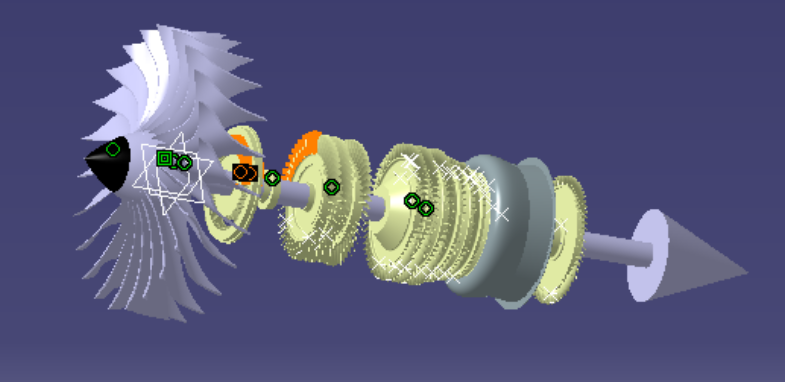
\includegraphics[width=0.9\textwidth]{4.png}
	\caption{Adittion of the combustor to the assembly.}
\end{figure}

Given the model of the combustor is such an irregular shape, ensuring the concentricity of the piece with the shaft is difficult as there isn't a defined radius in the combustor. A way of getting around this is by using the planes in the combustor and the planes in the shaft. As seen in figure 6, the three planes of the shaft are locked in place with the planes of the combustor. They are overlapping, but the locked planes are the xy and the zx planes. Choosing these planes leaves us with just one degree of freedom which is the movement in the y-axis. We left out the rotation with respect to the shaft axis because the combustor doesn't need to rotate.
\subsubsection*{Turbine}

At the turbine stage, we can see in figure 1 that the air is expanded and therefore, its energy will make the turbine rotate. In this design we have two phases in the turbine stage, the high pressure turbine and the low pressure turbine. The way the orientation of the turbine is determined is by their blades. The blades should be facing the opposite way the blades of the compressor are facing. This is to make the air blast into the surface of these blades and by Newton's third law of motion, get them moving. All the air and residue gases flow to the exhaust and are disposed.

Finding the right orientation of the turbines the constrains left are easy to define. Concentricity with the shaft will leave us with the same two degrees of liberty as the compressor, bearing and planetary assembly.

\begin{figure}[H]
	\centering
	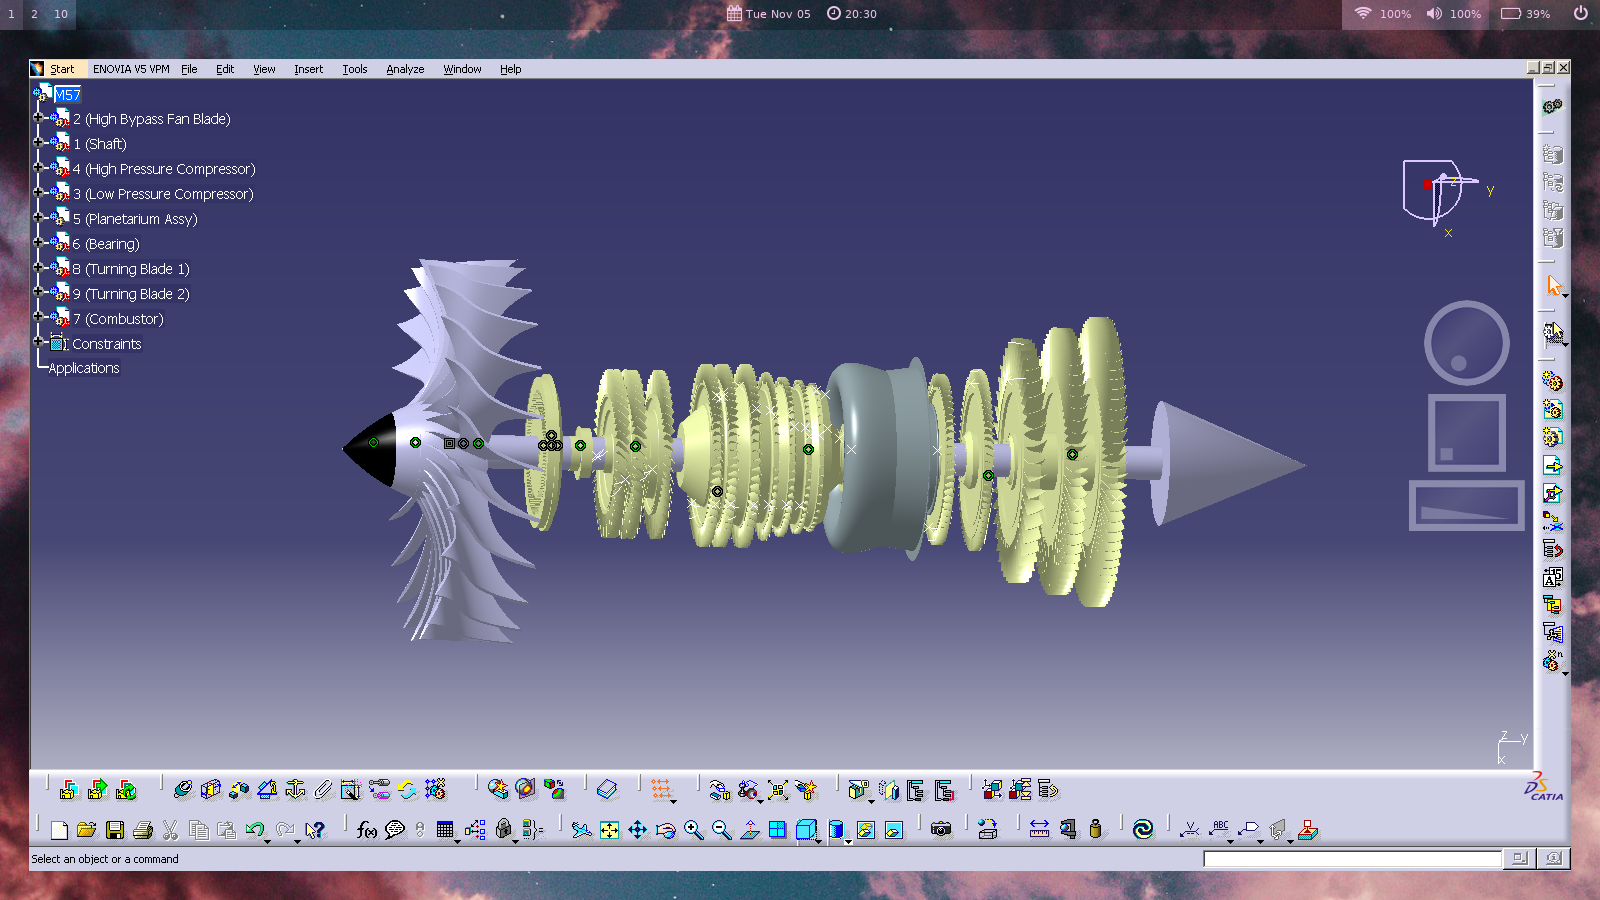
\includegraphics[width=\textwidth]{5.png}
	\caption{Turbines added to the assembly.}
\end{figure}

\section*{Conclusion}

After getting the assembly and constraining the different components, there's still a degree of freedom which needs to be restrained. The movement along the y-axis is undesired as we have mentioned before. To make this happen, it's necesarry to define the distances with respect to one piece of the assembly. In this case, the piece chosen as the reference is the fan blade. In particular, one fo the faces of the fan blade. The distances made where the following ones:

\begin{itemize}
	\item From the fan blade to the planetary assembly: 7.8 in.
	\item From the fan blade to the low pressure compressor: 12.15 in.
	\item From the fan blade to the high pressure compressor: 27.5 in.
	\item From the bearing to the compressor: 2.2 in (the compressor has its distance already defined, so the bearing will be defined aswell).
	\item From the fan blade to the high pressure turbine: 65.4 in.
	\item From the fan blade to the low pressure turbine: 74.8 in.
\end{itemize}

\begin{figure}[H]
	\centering
	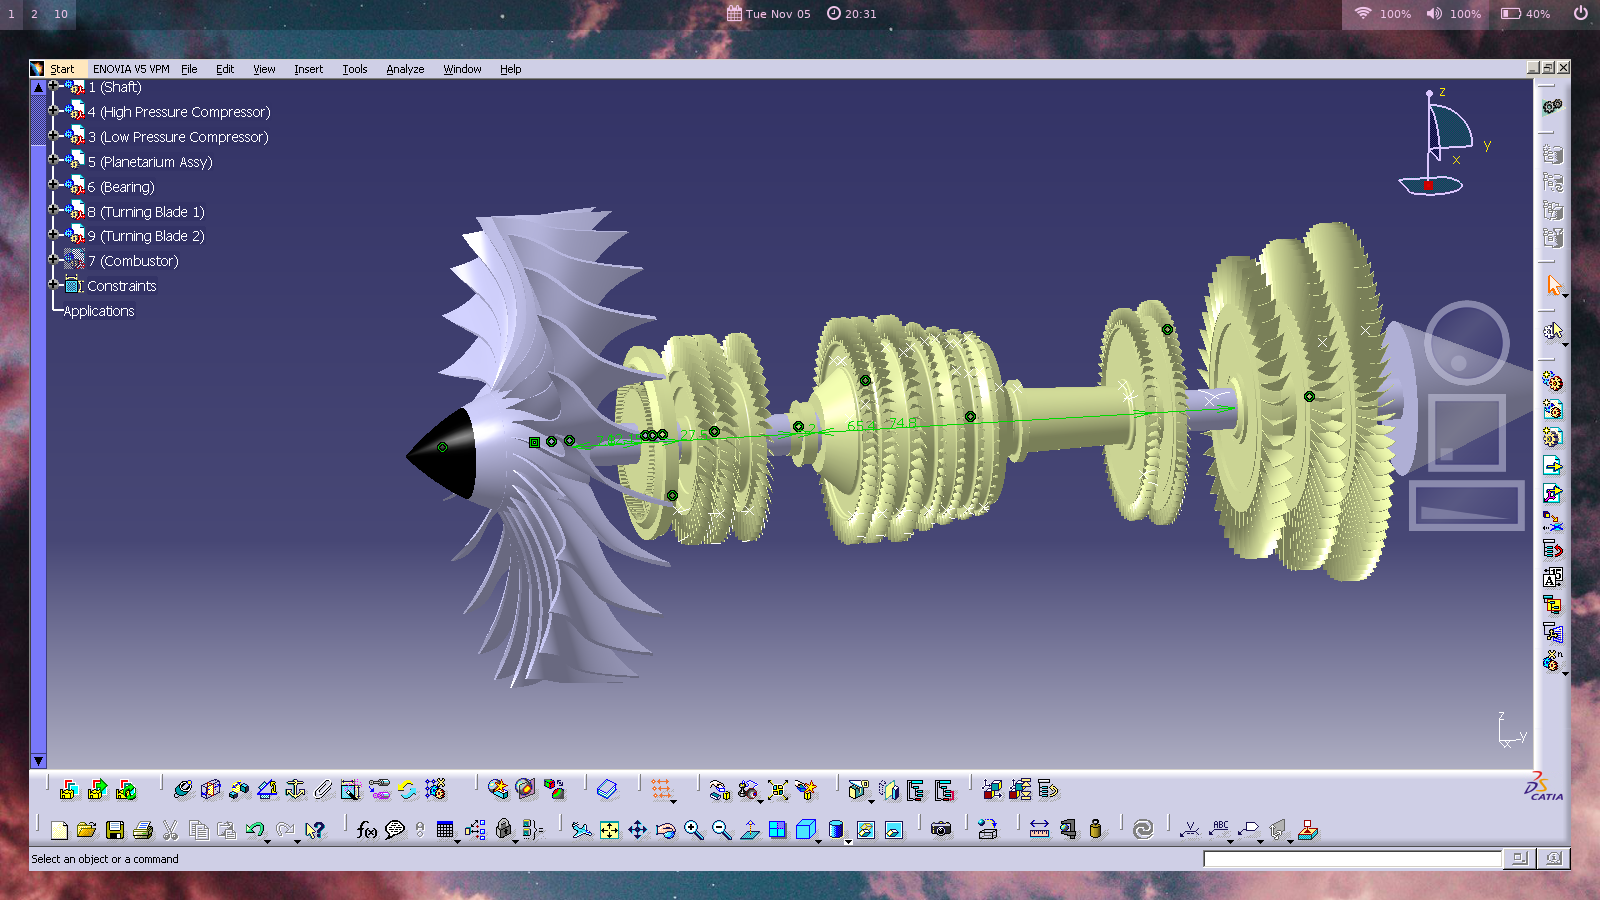
\includegraphics[width=\textwidth]{6.png}
	\caption{Whole assembly without the combustor, fully constrained.}
\end{figure}

There are a couple of point to be made. First, the combustor wasn't constrained as we didn't have much time left. Second, the bearing ended up between the low pressure and high pressure compressor.

After having made the whole assembly, it is certain that by knowing how each part operates and how the engine overall works it is easier to make a succesful assembly. If the knowledge of the individual pieces wasn't available, the considerations we have made with the orientation of blades would have been totally random, with the uncertainty of whether the engine would have worked or not.

We can conclude that any assembly and design is made more efficiently and we can assure its optimal functions knowing how it operates. 
%%%%%  Bib
\renewcommand\refname{References}
\begin{thebibliography}{}

	\bibitem[1]{n1}NASA, \textit{Gas Turbine Propulsion}, \textsc{\textbf{url:}} \url{https://www.grc.nasa.gov/WWW/K-12/airplane/Animation/turbtyp/etfp.html}.

	\bibitem[2]{n2}NASA, \textit{Combustor-Burner}, \textsc{\textbf{url:}} \url{https://www.grc.nasa.gov/WWW/K-12/airplane/burner.html}.

	\bibitem[3]{n3}NASA, \textit{Compressors}, \textsc{\textbf{url:}} \url{https://www.grc.nasa.gov/www/K-12/airplane/compress.html}.

	\bibitem[4]{n3}Nagpurwala, Q.H.,  \textit{Design of Gas Turbine Combustors}, \textsc{\textbf{url:}} \url{http://164.100.133.129:81/econtent/Uploads/12\%20PT12-Combustor\%2061\%20\%5BCompatibility\%20Mode\%5D.pdf}.

\end{thebibliography}
%\printbibliography
\end{document}
